\documentclass[12pt]{ctexart}  
% 官方要求字号不小于12
\CTEXsetup[format={\Large\bfseries}]{section} %在ctexart中,一级标题是居中的,这里改成左对齐

% 请在以下的方括号中填写队伍控制号
\usepackage[number]{ldmcm}  % 载入ldmcm模板文件
\problem{E}  % 请在此处填写题号

% 字体选择
% \usepackage{mathptmx}  % 这是 Times 字体,中规中矩 
\usepackage{mathpazo}  % 这是 COMAP 官方杂志采用的字体

% 几处小修改,如无特殊需求可不做更改
\newcommand{\upcite}[1]{\textsuperscript{\textsuperscript{\cite{#1}}}}%这是参考文献引用上标的命令
\graphicspath{{img/}}          % 此处{img/}为相对路径,注意加上“/”
\let\itemize\compactitem
\let\enditemize\endcompactitem %解决列表环境中行距过大的问题

\title{Sustainability of Insurance under Natural Disasters \\ Caused by Climate Change}  % 标题
% 修改题头,默认为 MCM /ICM
\renewcommand{\contest}{ICM}

% ----------------------------------------------文档开始---------------------------------------------------------
\begin{document}

% 此处填写摘要内容
\begin{abstract}
	%第一段:2句话背景+2句话概括全文完成的任务
	With the emergence of various extreme climates,\textbf{Austral-ia's wildfires} 

	%第二段:总结我们用了什么模型
	Several models are established: 

	%接下来分别介绍模型与结果
	For Model I:
	Firstly,%首先,我们从哪里收集到了什么样的数据
	We find data...
	Then,%然后,基于什么样的原因,我们建立了什么模型
	we establish \textbf{model}...
	Next,%我们选择或者设计了什么算法
	we use Algorithm...
	Finally,%我们得到了什么样的结果
	%数值直接写出来,大量数据(表)或图片则说请参见(are shown in ...)图几
	%注意要用文字,不要使用符号
	it can be seen that ...

	For Model II:
	Firstly,%首先,我们从哪里收集到了什么样的数据
	We find data...
	Then,%然后,基于什么样的原因,我们建立了什么模型
	we establish model...
	Next,%我们选择或者设计了什么算法
	we use Algorithm...
	Finally,%我们得到了什么样的结果
	%数值直接写出来,大量数据(表)或图片则说请参见(are shown in ...)图几
	%注意要用文字,不要使用符号
	it can be seen that...

	%灵敏度与稳健性分析
	Finally, sensitivity analysis ... Meanwhile, robustness

	% 美赛论文中无需注明关键词。若一定要使用,
	% 请将以下两行的注释号 '%' 去除,以使其生效
	%\vspace{5pt}
	%\textbf{Keywords}: MATLAB, mathematics, LaTeX.

\end{abstract}

\maketitle  % 生成 Summary Sheet------------------------------------

\tableofcontents  % 生成目录


% -----------------------------------------正文开始-----------------------------------------------------------------------------------------------------------------------------------


%==============第一部分===引入=============================================================
\section{Introduction}
\subsection{Problem Background}%问题背景---------------------------------
Extreme-weather events are becoming a crisis for property owners and insurers. 
The world has endured “more than \$1 trillion in damages from more than 1,000 extreme-weather events in recent years.”
The insurance industry saw claims for natural disasters in 2022 increase by “115\% compared to the 30-year average.” 
Conditions are expected to get worse as losses from severe weather-related events are likely to increase 
due to floods, hurricanes, cyclones, droughts, and wildfires. 
Premiums for insurance coverage are rising quickly, 
with climate change fueling projected increases of 30-60\% by 2040.

Property insurance is not only getting more expensive, 
but also harder to find, 
as insurance companies change how and where they are willing to underwrite policies. 
The weather-related occurrences propelling the cost of property insurance premiums look different depending on where you are in the world. 
Additionally, the insurance protection gap averages 57\% worldwide and is increasing.
This highlights the industry’s dilemma
- the emerging crisis in profitability for the insurers and in affordability for the property owners.


\subsection{Problem Restatement}% 问题重述----------
% \subsection{Literature Review} % 文献综述----------
Four major problems are discussed in this paper, which are:
\begin{itemize}
	\item determine whether the insurance model should be covered in areas 
	where the frequency of natural disasters increase.
	\item use the previous insurance model to guide real-estate 
	and offer appropriate services to growing communities and populations.
	\item measure a historic building and allocate conservation energy 
	based on cultural, historical, economic and community significance.
	\item need to write a letter which contains both future plan, schedule and cost,
	based on the Insurance Model and the Value model
\end{itemize}
A literatrue\upcite{kopka2003guide} says something about this problem ...



\subsection{Our work}%-----------------------------------------------------------
We do such things ...
这部分直接上图

美赛一定要多上图,清晰直观,并且格式上最好是矢量图,例如pdf,而不是位图,例如jpg,png等,在形式上最好是组图,下面列出了利用\verb|subfigure|实现的
\verb|1x2,1x3,2x2|的几种组图:

%% 这是一个1x2的组图
\begin{figure}[htbp]
	\centering
	\begin{subfigure}[b]{.3\textwidth} %设置缩放比例,这里的.5代表缩放为原来的50%
		
\includegraphics[width=\textwidth]{img/example-image-a.pdf}
		\caption{left}\label{subfig:left}
	\end{subfigure}
	\hspace{10mm} %%%%%%%%%%%%%%%%%%调整子图间距
	\begin{subfigure}[b]{.3\textwidth}
		
\includegraphics[width=\textwidth]{img/example-image-b.pdf}
		\caption{right}\label{subfig:right}
	\end{subfigure}
	\caption{Two images}\label{subfigure}
\end{figure}

Figure \ref{subfigure} gives an example of subfigures. Figure \ref{subfig:left} is on the left, and Figure \ref{subfig:right} is on the right.


%% 这是一个1x3的组图
\begin{figure}[!htbp]
	\centering
	\begin{subfigure}[t]{0.3\textwidth}
		\centering
		
\includegraphics[width=\textwidth]{img/example-image-a.pdf}
		\caption*{}
		\label{}
	\end{subfigure}
	\begin{subfigure}[t]{0.3\textwidth}
		\centering
		
\includegraphics[width=\textwidth]{img/example-image-b.pdf}
		\caption*{}
		\label{}
	\end{subfigure}
	\begin{subfigure}[t]{0.3\textwidth}
		\centering
		
\includegraphics[width=\textwidth]{img/example-image-c.pdf}
		\caption*{}
		\label{}
	\end{subfigure}
	\caption{Three images}
	\label{Three images}
\end{figure}


%% 这是一个2x2的组图(可推广至2x3,3x3等)
\begin{figure}[!htbp]
	\centering
	\begin{subfigure}[t]{0.4\textwidth}
		\centering
		
\includegraphics[width=\textwidth]{img/example-image-a.pdf}
		\caption{左上}
		\label{}
	\end{subfigure}
	\begin{subfigure}[t]{0.4\textwidth}
		\centering
		
\includegraphics[width=\textwidth]{img/example-image-b.pdf}
		\caption{右上}
		\label{}
	\end{subfigure}
	%  \begin{subfigure}[t]{0.3\textwidth}
	%          \centering
	%          
\includegraphics[width=\textwidth]{img/example-image-a.pdf.pdf}
	%          \caption{}
	%          \label{}
	%  \end{subfigure}
	\qquad
	%%让图片换行,这就是实现多行组图的简单原理
%%若需要搞一个2x3的组图就把上下的注释打开再添加图片就可以了
%%注意调整比例以及间距
	\begin{subfigure}[t]{0.4\textwidth}
		\centering
		
\includegraphics[width=\textwidth]{img/example-image-a.pdf}
		\caption{左下}
		\label{}
	\end{subfigure}
	\begin{subfigure}[t]{0.4\textwidth}
		\centering
		
\includegraphics[width=\textwidth]{img/example-image-b.pdf}
		\caption{右下}
		\label{}
	\end{subfigure}
	%\begin{subfigure}[t]{0.3\textwidth}
	%        \centering
	%        \includegraphics[width=\textwidth]{img/npca13.pdf}
	%        \caption{result}
	%        \label{}
	%\end{subfigure}
	\caption{组图组图变变变}
\end{figure}


\begin{enumerate}[\bfseries 1.]
	\item We do ...
	\item We do ...
	\item We do ...
\end{enumerate}

%===========================第二部分==模型准备==========================================================
\section{Preparation of the Models}
\subsection{Assumptions and Explanations}

%为了简化问题,我们做出了以下假设,其中每一条都有对应的合理解释
To simplify the problem, we made the following assumptions, each of which has a corresponding reasonable explanation.
\begin{itemize}
	\item \textit{\textbf{Assumption 1:}}假设\\$\hookrightarrow$ \textit{\textbf{Explanation:}}理由

	\item \textit{\textbf{Assumption 2:}}假设\\$\hookrightarrow$ \textit{\textbf{Explanation:}}理由

	\item \textit{\textbf{Assumption 3:}}假设\\$\hookrightarrow$ \textit{\textbf{Explanation:}}理由

	\item \textit{\textbf{Assumption 4:}}假设\\$\hookrightarrow$ \textit{\textbf{Explanation:}}理由
\end{itemize}
%这里只列出了主要的假设,其他假设会在专门的小节中单独讨论
Additional assumptions are made to simplify analysis for individual sections. These assumptions will be discussed at the appropriate locations.

% \newpage
\subsection{Notations}%-----------------------------------------------------------------------------------
% 三线表(可以直接在excel里编辑好然后用excel2latex插件插入)

Table \ref{tb:notation} lists some important mathematical notations used in this paper.
\begin{table}[htbp]%----------------------------------------------
	\begin{center}
		\caption{Notations used in this paper}
		\begin{tabular}{cl}
			\toprule[1.5pt]
			\multicolumn{1}{m{4cm}}{\centering \textbf{Symbol}}
			                      & \multicolumn{1}{m{10cm}}{\textbf{ Description} }                       \\
			\midrule
			$x_i$                 & Longitude within the i-th Wildfire Grid                                \\
			$y_i$                 & Latitude within the i-th Wildfire Grid                                 \\
			$\varOmega _i$        & The area of the i-th grid                                              \\
			$d_{ki}$              & the distance $d_{ki}$                                                  \\
			$SC_k$                & Score for evaluating the k-th wildfire grid                            \\
			\vspace{5pt}%公式间有点挤,空一些
			$x^{( \alpha )}_{ki}$ & the $SSA_\alpha$ drone sent by the k-th EOC to the i-th wild-fire grid \\
			\vspace{3pt}
			$x^{( \beta )}_{ki}$  & the $RR_\beta$ drone sent by the k-th EOC to the i-th wildfire grid    \\
			$t_{fly}^{\delta}$    & The flight time of drones                                              \\
			\bottomrule[1.5pt]
		\end{tabular}\label{tb:notation}
		\begin{tablenotes}
			\footnotesize
			\item[*] *Some variables are not listed here and will be discussed in detail in each section. %此处加入注释*信息
		\end{tablenotes}
	\end{center}
\end{table}
\vspace{-1cm}%在\end{table}下加一行\vspace{-1cm} 其中-1的作用是缩短与下方文字距离的 切记!必须是负数



%数据处理------------------------------------------------------------------------


\subsection{Data}
\subsubsection{Data Collection}
%下面列出了我们收集数据的来源网站
Websites, where we collect data, are listed in Table \ref{tb:data}.

\begin{table}[htbp]%----------------------------------------------
	\begin{center}
		\caption{Notations used in this paper}
		\begin{tabular}{c c}
			\toprule[1.5pt]
			\multicolumn{1}{m{5cm}}{\centering \textbf{Database Names}}
			               & \multicolumn{1}{m{10cm}}{\centering \textbf{Database Websites}}   \\
			\midrule
			Google Scholar & \href{https://scholar.google.com} {https://scholar.google.com}    \\
			Wikipedia      & \href{https://www.wikipedia.org}{https://www.wikipedia.org}       \\
			wolframalpha   & \href{https://www.wolframalpha.com}{https://www.wolframalpha.com} \\
			\bottomrule[1.5pt]
		\end{tabular}\label{tb:data}
	\end{center}
\end{table}
\vspace{-1cm}%在\end{table}下加一行\vspace{-1cm} 其中-1的作用是缩短与下方文字距离的 切记!必须是负数

\subsubsection{Data Processing}

%=================================第三部分====================================================================
\section{Probelm}
\subsection{Probelm 1}
\subsubsection{Under what conditions should insurance companies underwrite policies?}

\begin{enumerate}[\bfseries 1.]
	\item Risk Assessment\\
	Risk assessment is a core activity for insurance companies, 
	involving the process of identifying, analyzing, and evaluating potential risks. 
	For extreme weather events, 
	this process is particularly complex due to the uncertainties brought about by climate change.
	Using technical methods and mathematical models to deal with the dynamic assessment risk of existing data.
	\item Pricing Strategy\\
	A dynamic pricing strategy allows insurance companies to adjust premiums 
	based on the results of risk assessments or other conditions 
	while a relatively stable price is necessary to establish a reputation.
	\item Risk Diversification\\
	Insurance companies can spread their underwritten risks, 
	reducing the potential for significant losses from a single disaster event.
	\item Collaboration\\
	Facing the challenges posed by climate change requires insurance companies 
	to collaborate with governments, businesses, and non-governmental organizations.
\end{enumerate}
Through these detailed measures, insurance companies can more effectively manage the risks posed by extreme weather events 
while ensuring the sustainable development and long-term profitability of their business.
\subsubsection{Details about Model 1}
The detail can be described by equation \eqref{eq:heat}:
\begin{equation}\label{eq:heat}
	\frac{\partial u}{\partial t} - a^2 \left( \frac{\partial^2 u}{\partial x^2} + \frac{\partial^2 u}{\partial y^2} + \frac{\partial^2 u}{\partial z^2} \right) = f(x, y, z, t)
\end{equation}

\subsection{Probelm 2}
\subsubsection{Details about this question}
The detail can be described by equation \eqref{eq:heat}:
\begin{equation}\label{eq:heat}
	\frac{\partial u}{\partial t} - a^2 \left( \frac{\partial^2 u}{\partial x^2} + \frac{\partial^2 u}{\partial y^2} + \frac{\partial^2 u}{\partial z^2} \right) = f(x, y, z, t)
\end{equation}

\subsection{Problem 3}
\subsubsection{Conclusion of Model 2}
The results are shown in Figure \ref{fig:result}, where $t$ denotes the time in seconds, and $c$ refers to the concentration of water in the boiler.

\begin{figure}[!ht]%---------------结果上图!!!!!!--------------
	\centering
	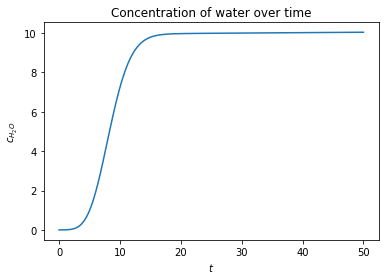
\includegraphics[width=.5\textwidth]{water.png}
	\caption{The result of Model 2}\label{fig:result}
\end{figure}%---------------------------------------------

伪代码,默认样式为\texttt{隐藏行号的三线表形式的伪代码}

%伪代码
\begin{algorithm}[H]
	\KwIn{输入}
	\KwOut{输出 }
	initialization\;
	\While{not at end of this document}{
		read current\;
		\Repeat{this end condition}{
			do these things\;
		}
		\eIf{understand}{
			go to next section\;
			current section becomes this one\;
		}{
			go back to the beginning of current section\;
		}
		\Do{this end condition}{
			do these things\;
		}
	}
	\caption{How to write algorithms}
\end{algorithm}
%伪代码%%%%%%%%%%%%%%%%%%%%%%

\clearpage
\subsubsection{Commetary on Model 2}
The instance of long and wide tables are shown in Table \ref{tb:longtable}.

% 长表格示例,更多用法请参考 longtable 宏包文档
% 以下环境及对应参数可实现表格内的自动换行与表格的自动断页
\begin{longtable}{ p{4em} p{14em} p{14em} }
	\caption{Basic Information about two Main Continents}
	\label{tb:longtable}                                                                                                                      \\
	\toprule
	Continent
	& Description 
	& Information \\
	\midrule
	North America
	& 1
	& 2 \\
	\midrule
	Asia
	& 3
	& 4 \\                                                                                               \\
	\bottomrule
\end{longtable}


%===============================================第四部分=============================================
\section{Test the Model}
\subsection{Sensitivity  Analysis}
\subsection{Robustness Analysis}
\texttt{这部分很重要,不能缺!}

%==============================================第五部分================================================
\section{Conclusion}
\subsection{Summary of Results}

\subsection{Strengths}%------------------优点----------------
\begin{itemize}
	%1. 有灵敏度分析与稳健性分析
	\item The sensitivity analysis of the model demonstrates the effectiveness of the model under different parameter combinations and prove the robustness of the mod
	\item Second one ...
\end{itemize}

\subsection{Weaknesses and Improvements}%---------------缺点与改进---------------------
\begin{itemize}
	\item The analysis of ... can be more accurate if we have more complete data;
	\item 123
\end{itemize}

% 可将整个 letter 环境移动到文章开头或中间
\begin{letter}{letter}
	\begin{flushleft}  % 左对齐环境,无首行缩进
		\textbf{To:} a historic landmark\\
		\textbf{From:} Team Number\\
		\textbf{Date:} February 5, 2024\\
		\textbf{Subject:} a letter to the community recommending a plan, timeline, and cost proposal 
		for the future of their treasured landmark
	\end{flushleft}
the contents of the letter...
\end{letter}

%=================================================================================================================

% 参考文献,直接把bib格式粘贴到References.bib里面,无需改动
\bibliographystyle{unsrt} %规定了参考文献的格式
\begin{center}
	\bibliography{references.bib} %调出LaTeX生成参考文献列表
\end{center}
%=====================================================================================

% 以下为附录内容
\begin{subappendices}  % 附录环境

	\section{Appendix A: something}

	\section{Appendix B: Program Codes}
	Here are the program codes we used in our research.

	% 代码环境示例

	% Python 代码示例
	\lstinputlisting[language=python]{code/example.py}

	% MATLAB 代码示例
	\lstinputlisting[language=matlab]{code/example.m}

\end{subappendices}  % 附录内容结束

\end{document}  % 结束
